\documentclass[12pt,a4paper]{article}

\usepackage[a4paper,text={16.5cm,25.2cm},centering]{geometry}
\usepackage{lmodern}
\usepackage{amssymb,amsmath}
\usepackage{bm}
\usepackage{graphicx}
\usepackage{microtype}
\usepackage{hyperref}
\setlength{\parindent}{0pt}
\setlength{\parskip}{1.2ex}

\hypersetup
       {   pdfauthor = { Marco Fasondini },
           pdftitle={ foo },
           colorlinks=TRUE,
           linkcolor=black,
           citecolor=blue,
           urlcolor=blue
       }




\usepackage{upquote}
\usepackage{listings}
\usepackage{xcolor}
\lstset{
    basicstyle=\ttfamily\footnotesize,
    upquote=true,
    breaklines=true,
    breakindent=0pt,
    keepspaces=true,
    showspaces=false,
    columns=fullflexible,
    showtabs=false,
    showstringspaces=false,
    escapeinside={(*@}{@*)},
    extendedchars=true,
}
\newcommand{\HLJLt}[1]{#1}
\newcommand{\HLJLw}[1]{#1}
\newcommand{\HLJLe}[1]{#1}
\newcommand{\HLJLeB}[1]{#1}
\newcommand{\HLJLo}[1]{#1}
\newcommand{\HLJLk}[1]{\textcolor[RGB]{148,91,176}{\textbf{#1}}}
\newcommand{\HLJLkc}[1]{\textcolor[RGB]{59,151,46}{\textit{#1}}}
\newcommand{\HLJLkd}[1]{\textcolor[RGB]{214,102,97}{\textit{#1}}}
\newcommand{\HLJLkn}[1]{\textcolor[RGB]{148,91,176}{\textbf{#1}}}
\newcommand{\HLJLkp}[1]{\textcolor[RGB]{148,91,176}{\textbf{#1}}}
\newcommand{\HLJLkr}[1]{\textcolor[RGB]{148,91,176}{\textbf{#1}}}
\newcommand{\HLJLkt}[1]{\textcolor[RGB]{148,91,176}{\textbf{#1}}}
\newcommand{\HLJLn}[1]{#1}
\newcommand{\HLJLna}[1]{#1}
\newcommand{\HLJLnb}[1]{#1}
\newcommand{\HLJLnbp}[1]{#1}
\newcommand{\HLJLnc}[1]{#1}
\newcommand{\HLJLncB}[1]{#1}
\newcommand{\HLJLnd}[1]{\textcolor[RGB]{214,102,97}{#1}}
\newcommand{\HLJLne}[1]{#1}
\newcommand{\HLJLneB}[1]{#1}
\newcommand{\HLJLnf}[1]{\textcolor[RGB]{66,102,213}{#1}}
\newcommand{\HLJLnfm}[1]{\textcolor[RGB]{66,102,213}{#1}}
\newcommand{\HLJLnp}[1]{#1}
\newcommand{\HLJLnl}[1]{#1}
\newcommand{\HLJLnn}[1]{#1}
\newcommand{\HLJLno}[1]{#1}
\newcommand{\HLJLnt}[1]{#1}
\newcommand{\HLJLnv}[1]{#1}
\newcommand{\HLJLnvc}[1]{#1}
\newcommand{\HLJLnvg}[1]{#1}
\newcommand{\HLJLnvi}[1]{#1}
\newcommand{\HLJLnvm}[1]{#1}
\newcommand{\HLJLl}[1]{#1}
\newcommand{\HLJLld}[1]{\textcolor[RGB]{148,91,176}{\textit{#1}}}
\newcommand{\HLJLs}[1]{\textcolor[RGB]{201,61,57}{#1}}
\newcommand{\HLJLsa}[1]{\textcolor[RGB]{201,61,57}{#1}}
\newcommand{\HLJLsb}[1]{\textcolor[RGB]{201,61,57}{#1}}
\newcommand{\HLJLsc}[1]{\textcolor[RGB]{201,61,57}{#1}}
\newcommand{\HLJLsd}[1]{\textcolor[RGB]{201,61,57}{#1}}
\newcommand{\HLJLsdB}[1]{\textcolor[RGB]{201,61,57}{#1}}
\newcommand{\HLJLsdC}[1]{\textcolor[RGB]{201,61,57}{#1}}
\newcommand{\HLJLse}[1]{\textcolor[RGB]{59,151,46}{#1}}
\newcommand{\HLJLsh}[1]{\textcolor[RGB]{201,61,57}{#1}}
\newcommand{\HLJLsi}[1]{#1}
\newcommand{\HLJLso}[1]{\textcolor[RGB]{201,61,57}{#1}}
\newcommand{\HLJLsr}[1]{\textcolor[RGB]{201,61,57}{#1}}
\newcommand{\HLJLss}[1]{\textcolor[RGB]{201,61,57}{#1}}
\newcommand{\HLJLssB}[1]{\textcolor[RGB]{201,61,57}{#1}}
\newcommand{\HLJLnB}[1]{\textcolor[RGB]{59,151,46}{#1}}
\newcommand{\HLJLnbB}[1]{\textcolor[RGB]{59,151,46}{#1}}
\newcommand{\HLJLnfB}[1]{\textcolor[RGB]{59,151,46}{#1}}
\newcommand{\HLJLnh}[1]{\textcolor[RGB]{59,151,46}{#1}}
\newcommand{\HLJLni}[1]{\textcolor[RGB]{59,151,46}{#1}}
\newcommand{\HLJLnil}[1]{\textcolor[RGB]{59,151,46}{#1}}
\newcommand{\HLJLnoB}[1]{\textcolor[RGB]{59,151,46}{#1}}
\newcommand{\HLJLoB}[1]{\textcolor[RGB]{102,102,102}{\textbf{#1}}}
\newcommand{\HLJLow}[1]{\textcolor[RGB]{102,102,102}{\textbf{#1}}}
\newcommand{\HLJLp}[1]{#1}
\newcommand{\HLJLc}[1]{\textcolor[RGB]{153,153,119}{\textit{#1}}}
\newcommand{\HLJLch}[1]{\textcolor[RGB]{153,153,119}{\textit{#1}}}
\newcommand{\HLJLcm}[1]{\textcolor[RGB]{153,153,119}{\textit{#1}}}
\newcommand{\HLJLcp}[1]{\textcolor[RGB]{153,153,119}{\textit{#1}}}
\newcommand{\HLJLcpB}[1]{\textcolor[RGB]{153,153,119}{\textit{#1}}}
\newcommand{\HLJLcs}[1]{\textcolor[RGB]{153,153,119}{\textit{#1}}}
\newcommand{\HLJLcsB}[1]{\textcolor[RGB]{153,153,119}{\textit{#1}}}
\newcommand{\HLJLg}[1]{#1}
\newcommand{\HLJLgd}[1]{#1}
\newcommand{\HLJLge}[1]{#1}
\newcommand{\HLJLgeB}[1]{#1}
\newcommand{\HLJLgh}[1]{#1}
\newcommand{\HLJLgi}[1]{#1}
\newcommand{\HLJLgo}[1]{#1}
\newcommand{\HLJLgp}[1]{#1}
\newcommand{\HLJLgs}[1]{#1}
\newcommand{\HLJLgsB}[1]{#1}
\newcommand{\HLJLgt}[1]{#1}



\def\qqand{\qquad\hbox{and}\qquad}
\def\qqfor{\qquad\hbox{for}\qquad}
\def\qqas{\qquad\hbox{as}\qquad}
\def\half{ {1 \over 2} }
\def\D{ {\rm d} }
\def\I{ {\rm i} }
\def\E{ {\rm e} }
\def\C{ {\mathbb C} }
\def\R{ {\mathbb R} }
\def\H{ {\mathbb H} }
\def\Z{ {\mathbb Z} }
\def\CC{ {\cal C} }
\def\FF{ {\cal F} }
\def\HH{ {\cal H} }
\def\LL{ {\cal L} }
\def\vc#1{ {\mathbf #1} }
\def\bbC{ {\mathbb C} }



\def\fR{ f_{\rm R} }
\def\fL{ f_{\rm L} }

\def\qqqquad{\qquad\qquad}
\def\qqwhere{\qquad\hbox{where}\qquad}
\def\Res_#1{\underset{#1}{\rm Res}\,}
\def\sech{ {\rm sech}\, }
\def\acos{ {\rm acos}\, }
\def\asin{ {\rm asin}\, }
\def\atan{ {\rm atan}\, }
\def\Ei{ {\rm Ei}\, }
\def\upepsilon{\varepsilon}


\def\Xint#1{ \mathchoice
   {\XXint\displaystyle\textstyle{#1} }%
   {\XXint\textstyle\scriptstyle{#1} }%
   {\XXint\scriptstyle\scriptscriptstyle{#1} }%
   {\XXint\scriptscriptstyle\scriptscriptstyle{#1} }%
   \!\int}
\def\XXint#1#2#3{ {\setbox0=\hbox{$#1{#2#3}{\int}$}
     \vcenter{\hbox{$#2#3$}}\kern-.5\wd0} }
\def\ddashint{\Xint=}
\def\dashint{\Xint-}
% \def\dashint
\def\infdashint{\dashint_{-\infty}^\infty}




\def\addtab#1={#1\;&=}
\def\ccr{\\\addtab}
\def\ip<#1>{\left\langle{#1}\right\rangle}
\def\dx{\D x}
\def\dt{\D t}
\def\dz{\D z}
\def\ds{\D s}

\def\rR{ {\rm R} }
\def\rL{ {\rm L} }

\def\norm#1{\left\| #1 \right\|}

\def\pr(#1){\left({#1}\right)}
\def\br[#1]{\left[{#1}\right]}

\def\abs#1{\left|{#1}\right|}
\def\fpr(#1){\!\pr({#1})}

\def\sopmatrix#1{ \begin{pmatrix}#1\end{pmatrix} }

\def\endash{–}
\def\emdash{—}
\def\mdblksquare{\blacksquare}
\def\lgblksquare{\blacksquare}
\def\scre{\E}
\def\mapengine#1,#2.{\mapfunction{#1}\ifx\void#2\else\mapengine #2.\fi }

\def\map[#1]{\mapengine #1,\void.}

\def\mapenginesep_#1#2,#3.{\mapfunction{#2}\ifx\void#3\else#1\mapengine #3.\fi }

\def\mapsep_#1[#2]{\mapenginesep_{#1}#2,\void.}


\def\vcbr[#1]{\pr(#1)}


\def\bvect[#1,#2]{
{
\def\dots{\cdots}
\def\mapfunction##1{\ | \  ##1}
	\sopmatrix{
		 \,#1\map[#2]\,
	}
}
}



\def\vect[#1]{
{\def\dots{\ldots}
	\vcbr[{#1}]
} }

\def\vectt[#1]{
{\def\dots{\ldots}
	\vect[{#1}]^{\top}
} }

\def\Vectt[#1]{
{
\def\mapfunction##1{##1 \cr}
\def\dots{\vdots}
	\begin{pmatrix}
		\map[#1]
	\end{pmatrix}
} }

\def\addtab#1={#1\;&=}
\def\ccr{\\\addtab}

\def\questionequals{= \!\!\!\!\!\!{\scriptstyle ? \atop }\,\,\,}

\begin{document}

\textbf{Applied Complex Analysis (2021)}

\section{Lecture 14: Inverting the Hilbert transform and ideal fluid flow}
In this lecture we

\begin{itemize}
\item[1. ] Discuss how to invert a Hilbert transform


\item[2. ] Use it to solve ideal fluid flow around a plate

\end{itemize}
\subsection{Inverting the Hilbert transform}
We now consider the problem of finding $u$ such that

\[
H_{[a,b]} u(x) = f(x)
\]
for $a < x < b$. Note that this is an additive jump problem: if we write $\phi(z) = \CC u(z)$ then we want to solve

\[
-\I (\phi_+(x) + \phi_-(x)) = f(x)
\]
where $\phi$ satisfies the conditions of Plemelj (Analyticity off $[a,b]$, weaker than pole singularities, decay at $\infty$). If we can find such a $\phi$, Plemelj guarantees that $u$ is recovered via

\[
\phi_+(x) - \phi_-(x) = (\CC^+ - \CC^-)u(x) = u(x)
\]
To tackle this we are going to reduce it to a subtractive problem. Writing

\[
\kappa(z) = \sqrt{z-a} \sqrt{z-b}
\]
which satisfies

\[
\kappa_+(x) = \I \sqrt{b-x} \sqrt{x-a} = -  \kappa_-(x)
\]
Thus if we write

\[
\phi(z) = { \psi(z) \over \kappa(z) }
\]
for some new unknown $\psi$ we have that

\[
f(x) = -\I (\phi_+(x) + \phi_-(x)) = -\I \left({\psi_+(x) \over \kappa_+(x)} + {\psi_-(x) \over \kappa_-(x)}\right) =
-\I {\psi_+(x) - \psi_-(x) \over \kappa_+(x)}
\]
In other words, we want

\[
\psi_+(x) - \psi_-(x) =  \I f(x) \kappa_+(x) = -f(x)\sqrt{b-x}\sqrt{x-a}
\]
where we need $\psi$ to be bounded (the decay of $1/\kappa$ then ensures the decay of $\phi$).  Therefore by Plemelj we have for $g(x) = f(x) \sqrt{b-x} \sqrt{x-a}$

\[
\psi(z) = -\CC g(z) - D
\]
and hence for


\begin{align*}
u(x) &= \phi_+(x) - \phi_-(x) = {\psi_+(x)\over \kappa_+(x)} - {\psi_-(x)\over \kappa_-(x)} \\
&= -{\CC^+ g(x) + \CC^- g(x) + 2 D \over \kappa_+(x)}
= -{\I \HH g(x) + 2D \over \kappa_+(x)}\\
& = -{\HH_{[a,b]}[f \sqrt{b-\diamond}\sqrt{\diamond-a}](x) + 2 D \over \sqrt{b-x} \sqrt{x-a}}
\end{align*}
where $\diamond$ denotes a dummy variable and $D$ is arbitrary.

In practice we determine $\HH g(x)$ by first computing its Cauchy transform.

\emph{Example} Let's try with $f(x) = x$ on $[-1,1]$. The first step is to compute the Cauchy transform of $g(x) = x \sqrt{1-x^2}$. Using the usual technique this gives

\[
\CC g(z) = {z \sqrt{z-1} \sqrt{z+1} - z^2 +1/2 \over 2 \I}
\]
where we use the Laurent series


\begin{align*}
\sqrt{z-1} \sqrt{z+1} &= z \sqrt{1-1/z} \sqrt{1 + 1/z} \ccr
= z (1+1/(2z) - 1/(8 z^2) + O(z^{-3}))(1-1/(2z)  - 1/(8 z^2) + O(z^{-3})) \ccr
= z -{1 \over 2 z} + O(z^{-2})
\end{align*}
Therefore


\begin{align*}
\HH g(x) &= -\I (\CC^+ + \CC^-) g(x) = - {x \sqrt{x-1}_+ \sqrt{x+1} - x \sqrt{x-1}_- \sqrt{x+1} \over 2} + x^2 - 1/2 \ccr
= x^2 - 1/2
\end{align*}
Giving us

\[
u(x) = -{x^2 - 1/2 + 2 D \over \sqrt{1-x^2}}
\]
Choosing $D = -1/4$ recovers the known solution $\sqrt{1-x^2}$.

\subsection{Ideal fluid flow}
Understanding branch cuts and Cauchy transforms allows us to systematically solve equations involving the Laplace equation. A classic example is ideal fluid flow. Consider the case of uniform flow with angle $\theta$ around an infinitesimally small plate on $[-1,1]$. We can model this as


\begin{align*}
v(x,y) &\sim y \cos \theta - x \sin \theta \qquad\hbox{as}\qquad x^2 + y^2 \to \infty  \\
v_{xx} + v_{yy} &= 0 \\
v(x,0) & = 0 \qqfor -1 < x <1
\end{align*}
Using the techniques we developed in the last few lectures, we obtain a nice, simple, closed form expression for the solution as the imaginary part of an analytic function:


\begin{lstlisting}
(*@\HLJLk{using}@*) (*@\HLJLn{Plots}@*)(*@\HLJLp{,}@*) (*@\HLJLn{LinearAlgebra}@*)(*@\HLJLp{,}@*) (*@\HLJLn{ApproxFun}@*)(*@\HLJLp{,}@*) (*@\HLJLn{SingularIntegralEquations}@*)
(*@\HLJLn{Cw}@*) (*@\HLJLoB{=}@*) (*@\HLJLp{(}@*)(*@\HLJLn{\ensuremath{\theta}}@*)(*@\HLJLp{,}@*)(*@\HLJLn{z}@*)(*@\HLJLp{)}@*) (*@\HLJLoB{->}@*) (*@\HLJLoB{-}@*)(*@\HLJLn{im}@*)(*@\HLJLoB{*}@*)(*@\HLJLnf{sin}@*)(*@\HLJLp{(}@*)(*@\HLJLn{\ensuremath{\theta}}@*)(*@\HLJLp{)}@*)(*@\HLJLoB{*}@*)(*@\HLJLp{(}@*)(*@\HLJLnf{sqrt}@*)(*@\HLJLp{(}@*)(*@\HLJLn{z}@*)(*@\HLJLoB{-}@*)(*@\HLJLni{1}@*)(*@\HLJLp{)}@*)(*@\HLJLnf{sqrt}@*)(*@\HLJLp{(}@*)(*@\HLJLn{z}@*)(*@\HLJLoB{+}@*)(*@\HLJLni{1}@*)(*@\HLJLp{)}@*) (*@\HLJLoB{-}@*) (*@\HLJLn{z}@*)(*@\HLJLp{)}@*)
(*@\HLJLn{\ensuremath{\varphi}}@*) (*@\HLJLoB{=}@*) (*@\HLJLp{(}@*)(*@\HLJLn{\ensuremath{\theta}}@*)(*@\HLJLp{,}@*)(*@\HLJLn{z}@*)(*@\HLJLp{)}@*) (*@\HLJLoB{->}@*) (*@\HLJLnf{exp}@*)(*@\HLJLp{(}@*)(*@\HLJLoB{-}@*)(*@\HLJLn{im}@*)(*@\HLJLoB{*}@*)(*@\HLJLn{\ensuremath{\theta}}@*)(*@\HLJLp{)}@*)(*@\HLJLoB{*}@*)(*@\HLJLn{z}@*) (*@\HLJLoB{+}@*) (*@\HLJLnf{Cw}@*)(*@\HLJLp{(}@*)(*@\HLJLn{\ensuremath{\theta}}@*)(*@\HLJLp{,}@*)(*@\HLJLn{z}@*)(*@\HLJLp{)}@*)
(*@\HLJLn{u}@*) (*@\HLJLoB{=}@*) (*@\HLJLp{(}@*)(*@\HLJLn{\ensuremath{\theta}}@*)(*@\HLJLp{,}@*)(*@\HLJLn{x}@*)(*@\HLJLp{,}@*)(*@\HLJLn{y}@*)(*@\HLJLp{)}@*) (*@\HLJLoB{->}@*) (*@\HLJLnf{imag}@*)(*@\HLJLp{(}@*)(*@\HLJLnf{\ensuremath{\varphi}}@*)(*@\HLJLp{(}@*)(*@\HLJLn{\ensuremath{\theta}}@*)(*@\HLJLp{,}@*) (*@\HLJLn{x}@*) (*@\HLJLoB{+}@*) (*@\HLJLn{im}@*)(*@\HLJLoB{*}@*)(*@\HLJLn{y}@*)(*@\HLJLp{))}@*)

(*@\HLJLn{xx}@*) (*@\HLJLoB{=}@*) (*@\HLJLn{yy}@*) (*@\HLJLoB{=}@*) (*@\HLJLnf{range}@*)(*@\HLJLp{(}@*)(*@\HLJLoB{-}@*)(*@\HLJLni{3}@*)(*@\HLJLp{;}@*) (*@\HLJLn{stop}@*)(*@\HLJLoB{=}@*)(*@\HLJLni{3}@*) (*@\HLJLp{,}@*) (*@\HLJLn{length}@*)(*@\HLJLoB{=}@*)(*@\HLJLni{500}@*)(*@\HLJLp{)}@*)
(*@\HLJLnf{contour}@*)(*@\HLJLp{(}@*)(*@\HLJLn{xx}@*)(*@\HLJLp{,}@*) (*@\HLJLn{yy}@*)(*@\HLJLp{,}@*) (*@\HLJLn{u}@*)(*@\HLJLoB{.}@*)(*@\HLJLp{(}@*)(*@\HLJLnfB{1.3}@*)(*@\HLJLp{,}@*)(*@\HLJLn{xx}@*)(*@\HLJLoB{{\textquotesingle}}@*)(*@\HLJLp{,}@*)(*@\HLJLn{yy}@*)(*@\HLJLp{);}@*) (*@\HLJLn{nlevels}@*) (*@\HLJLoB{=}@*) (*@\HLJLni{100}@*)(*@\HLJLp{)}@*)
(*@\HLJLnf{plot!}@*)(*@\HLJLp{(}@*)(*@\HLJLnf{Segment}@*)(*@\HLJLp{(}@*)(*@\HLJLoB{-}@*)(*@\HLJLnfB{1.}@*)(*@\HLJLp{,}@*)(*@\HLJLnfB{1.}@*)(*@\HLJLp{);}@*) (*@\HLJLn{color}@*)(*@\HLJLoB{=:}@*)(*@\HLJLn{black}@*)(*@\HLJLp{,}@*) (*@\HLJLn{label}@*)(*@\HLJLoB{=}@*)(*@\HLJLs{"{}obstacle"{}}@*)(*@\HLJLp{)}@*)
\end{lstlisting}

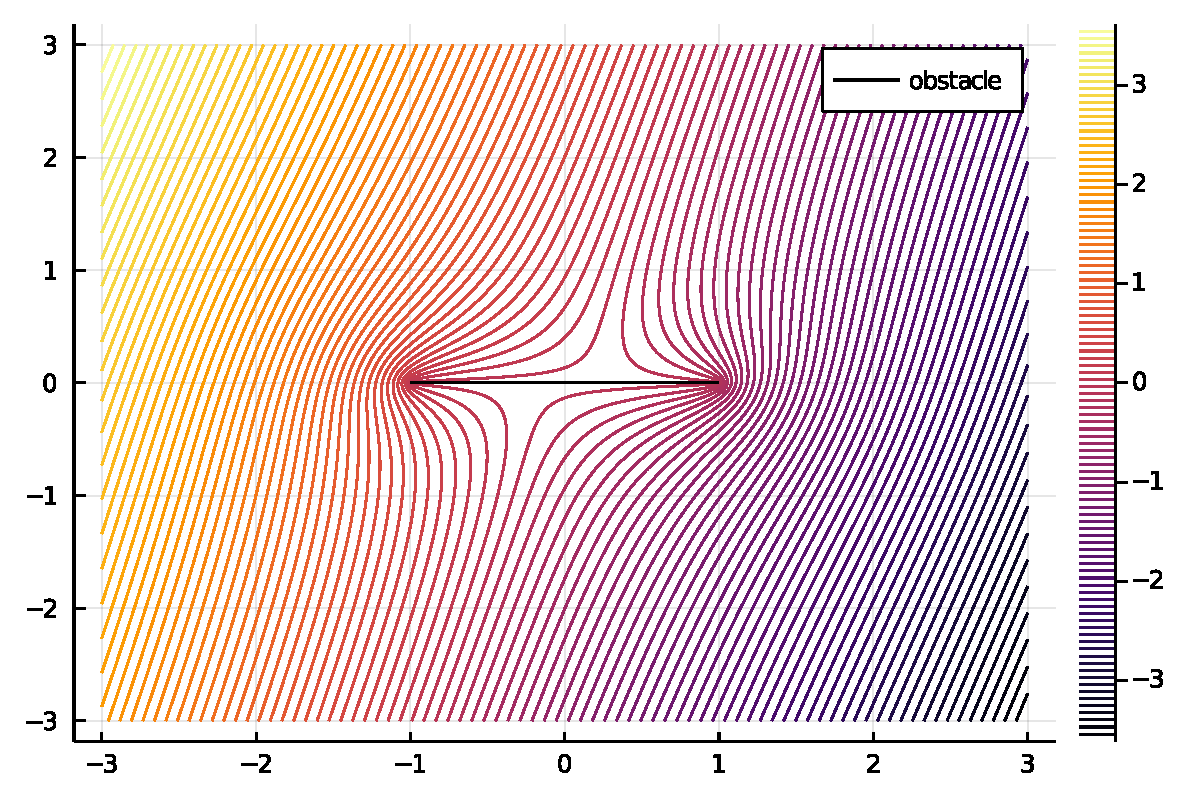
\includegraphics[width=\linewidth]{C:/Users/mfaso/OneDrive/Documents/GitHub/M3M6AppliedComplexAnalysis/output/figures/Lecture14_1_1.pdf}

We divide this task into stages:

\begin{itemize}
\item[1. ] Rephrasing as a complex-analytical problem: $v(x,y)$ to $\phi(z)$


\item[2. ] Reduction to inverting a Hilbert transform: $\phi(z)$ to $w(x)$


\item[3. ] Calculating the inverse Hilbert transform: Finding $w(x)$


\item[4. ] Calculating its Cauchy transform: $w(x)$ to $\phi(z)$

\end{itemize}
\subsubsection{Real and imaginary parts of analytic functions satisfy Laplace's equation}
The real and imaginary parts of an analytic function satisfy Laplace's equation: that is  if $\phi(z) = \phi(x + \I y) = u(x,y) + \I v(x,y)$ where $u$ and $v$ are the real/imaginary parts, then


\begin{align*}
 u_{xx} + u_{yy}&= 0 \\
 v_{xx} + v_{yy} &= 0
\end{align*}
To see this, note that the complex-derivative of $\phi(z)$ can be written in terms of two different partial derivatives:


\begin{align*}
    \phi'(z) &= \lim_{h \rightarrow 0} {\phi(z+h) - \phi(z) \over h} = \lim_{h \rightarrow 0} {u(x+h,y)-u(x,y) + \I (v(x+h,y)-v(x,y)) \over h} = u_x + \I v_x \ccr
    \phi'(z) = \lim_{h \rightarrow 0} {\phi(z+\I h) - \phi(z) \over \I h} = \lim_{h \rightarrow 0} {u(x,y+h)-u(x,y) + \I (v(x,y+h)-v(x,y)) \over \I h} = - \I u_y + v_y
\end{align*}
Taking a second derivative we get two equations:

\[
    \phi''(z) = u_{xx} + \I v_{xx} = -u_{yy} -\I v_{yy}
\]
which implies $u_{xx} + u_{yy} = 0$ and $v_{xx} + v_{yy} = 0$.

\subsubsection{2. Reduce PDE to the Hilbert transform of an unknown function}
Therefore we can rewrite the ideal fluid flow equation as a problem of calculating $\phi(z) = u(x,y) + \I v(x,y)$ whose imaginary part is the solution to the ideal fluid flow PDE (we don't use the real part $u$). That is, we want to find analytic $\phi(z)$ that satisfies


\begin{align*}
    \phi(z) &\sim \E^{-\I \theta} z \qquad\hbox{as}\qquad z \to \infty \\
    \Im \phi(x) &= 0  \qquad\hbox{for}\qquad -1 < x < 1
\end{align*}
Write

\[
\phi(z) = \E^{-\I \theta} z + c + \CC_{[-1,1]} w(z)
\]
for an as-of-yet unknown function $w$ and $c$ an unknown constant, we have (assuming $w$ is real) that

\[
0 = \Im \phi(x) = -x \sin \theta + \Im c + \Im \CC_{[-1,1]}^+ w(x) = -x \sin \theta + \Im c +{1 \over 2} \HH w(x)
\]
In this example, we can take $c = 0$. Therefore, we want to solve

\[
\HH w(x) =  2 x  \sin \theta
\]
for $w$.

\subsubsection{3. Calculating the inverse Hilbert transform}
We now plug the problem into the inverse Hilbert transform formula:

\[
    w(x) = {- 1\over \sqrt{1-x^2}} {\cal H}[f \sqrt{1-\diamond^2}](x)  + {D \over \sqrt{1-x^2}}
\]
where $f(x) = 2 x \sin \theta$. As we found before,

\[
{\cal C}[\diamond \sqrt{1-\diamond^2}](z) = {z \sqrt{z-1} \sqrt{z+1} - z^2 + 1/2 \over 2 \I }
\]
and therefore

\[
{\cal H}[\diamond \sqrt{1-\diamond^2}](x) = -\I({\cal C}^+ + {\cal C}^-)[\diamond \sqrt{1-\diamond^2}](x) = x^2 - {1 \over 2}
\]
Thus (relabeling $D$) we have

\[
w(x) = 2\sin \theta {D - x^2 \over \sqrt{1-x^2}}
\]
\emph{Demonstration} Here we see that this gives us the right Hilbert transform:


\begin{lstlisting}
(*@\HLJLn{D}@*) (*@\HLJLoB{=}@*) (*@\HLJLnf{randn}@*)(*@\HLJLp{()}@*)
(*@\HLJLn{\ensuremath{\theta}}@*) (*@\HLJLoB{=}@*) (*@\HLJLnfB{0.1}@*)
(*@\HLJLn{x}@*) (*@\HLJLoB{=}@*) (*@\HLJLnf{Fun}@*)(*@\HLJLp{()}@*)
(*@\HLJLn{w}@*) (*@\HLJLoB{=}@*) (*@\HLJLni{2}@*)(*@\HLJLnf{sin}@*)(*@\HLJLp{(}@*)(*@\HLJLn{\ensuremath{\theta}}@*)(*@\HLJLp{)}@*) (*@\HLJLoB{*}@*) (*@\HLJLp{(}@*)(*@\HLJLn{D}@*)(*@\HLJLoB{-}@*)(*@\HLJLn{x}@*)(*@\HLJLoB{{\textasciicircum}}@*)(*@\HLJLni{2}@*)(*@\HLJLp{)}@*)(*@\HLJLoB{/}@*)(*@\HLJLnf{sqrt}@*)(*@\HLJLp{(}@*)(*@\HLJLni{1}@*)(*@\HLJLoB{-}@*)(*@\HLJLn{x}@*)(*@\HLJLoB{{\textasciicircum}}@*)(*@\HLJLni{2}@*)(*@\HLJLp{)}@*)
(*@\HLJLoB{-}@*)(*@\HLJLnf{hilbert}@*)(*@\HLJLp{(}@*)(*@\HLJLn{w}@*)(*@\HLJLp{,}@*)(*@\HLJLnfB{0.2}@*)(*@\HLJLp{)}@*) (*@\HLJLp{,}@*) (*@\HLJLni{2}@*)(*@\HLJLnf{sin}@*)(*@\HLJLp{(}@*)(*@\HLJLn{\ensuremath{\theta}}@*)(*@\HLJLp{)}@*)(*@\HLJLoB{*}@*)(*@\HLJLnfB{0.2}@*) (*@\HLJLcs{{\#}}@*) (*@\HLJLcs{Minus}@*) (*@\HLJLcs{in}@*) (*@\HLJLcs{front}@*) (*@\HLJLcs{of}@*) (*@\HLJLcs{w}@*) (*@\HLJLcs{to}@*) (*@\HLJLcs{fix}@*) (*@\HLJLcs{normalisation}@*)
\end{lstlisting}

\begin{lstlisting}
(0.03993336665873126, 0.03993336665873126)
\end{lstlisting}


\[
D
\]
is arbitrary, but from physical principles we know that we don't want the solution to blow up. If $w$ blows up then so does its Cauchy transform. Therefore, we choose $D = 1$ so that

\[
w(x) = 2 \sin \theta \sqrt{1-x^2}
\]
\subsubsection{4. Calculating its Cauchy transform}
Now recall

\[
\CC\left[{\sqrt{1-\diamond^2}}\right](z) = {\sqrt{z-1} \sqrt{z+1} -z \over 2 \I}
\]
Therefore, $w(x) = 2 \sin \theta \sqrt{1-x^2}$,  implies

\[
\CC w(z) = - \I \sin \theta (\sqrt{z-1} \sqrt{z+1} -z)
\]
which means

\[
\phi(z) = \E^{-\I \theta} z - \I \sin \theta (\sqrt{z-1} \sqrt{z+1} -z).
\]
\subsection{Numerical example of two intervals}
We note that for obstacles on the real line, represented by a contour $\Gamma$, the problem of ideal fluid flow around $\Gamma$ is still reducible to solving the singular integral equation

\[
\HH_\Gamma f(x) = 2 x  \sin \theta
\]
Even when not solvable exactly, one can solve it numerically:


\begin{lstlisting}
(*@\HLJLn{a}@*) (*@\HLJLoB{=}@*) (*@\HLJLnfB{0.3}@*)
(*@\HLJLn{\ensuremath{\theta}}@*) (*@\HLJLoB{=}@*) (*@\HLJLnfB{1.3}@*)
(*@\HLJLn{\ensuremath{\Gamma}}@*) (*@\HLJLoB{=}@*) (*@\HLJLnf{Segment}@*)(*@\HLJLp{(}@*)(*@\HLJLoB{-}@*)(*@\HLJLni{1}@*)(*@\HLJLp{,}@*)(*@\HLJLoB{-}@*)(*@\HLJLn{a}@*)(*@\HLJLp{)}@*) (*@\HLJLoB{\ensuremath{\cup}}@*) (*@\HLJLnf{Segment}@*)(*@\HLJLp{(}@*)(*@\HLJLn{a}@*)(*@\HLJLp{,}@*) (*@\HLJLni{1}@*)(*@\HLJLp{)}@*)

(*@\HLJLn{x}@*) (*@\HLJLoB{=}@*) (*@\HLJLnf{Fun}@*)(*@\HLJLp{(}@*)(*@\HLJLn{\ensuremath{\Gamma}}@*)(*@\HLJLp{)}@*)
(*@\HLJLn{sp}@*) (*@\HLJLoB{=}@*) (*@\HLJLnf{PiecewiseSpace}@*)(*@\HLJLp{(}@*)(*@\HLJLn{JacobiWeight}@*)(*@\HLJLoB{.}@*)(*@\HLJLp{(}@*)(*@\HLJLnfB{0.5}@*)(*@\HLJLp{,}@*)(*@\HLJLnfB{0.5}@*)(*@\HLJLp{,}@*)(*@\HLJLnf{components}@*)(*@\HLJLp{(}@*)(*@\HLJLn{\ensuremath{\Gamma}}@*)(*@\HLJLp{))}@*)(*@\HLJLoB{...}@*)(*@\HLJLp{)}@*)
(*@\HLJLn{H}@*) (*@\HLJLoB{=}@*) (*@\HLJLnf{Hilbert}@*)(*@\HLJLp{(}@*)(*@\HLJLn{sp}@*)(*@\HLJLp{)}@*)

(*@\HLJLn{o{\_}1}@*) (*@\HLJLoB{=}@*) (*@\HLJLnf{Fun}@*)(*@\HLJLp{(}@*)(*@\HLJLn{x}@*) (*@\HLJLoB{->}@*) (*@\HLJLoB{-}@*)(*@\HLJLni{1}@*) (*@\HLJLoB{\ensuremath{\leq}}@*) (*@\HLJLn{x}@*) (*@\HLJLoB{\ensuremath{\leq}}@*) (*@\HLJLoB{-}@*)(*@\HLJLn{a}@*) (*@\HLJLoB{?}@*) (*@\HLJLni{1}@*) (*@\HLJLoB{:}@*) (*@\HLJLni{0}@*)(*@\HLJLp{,}@*) (*@\HLJLn{\ensuremath{\Gamma}}@*) (*@\HLJLp{)}@*)
(*@\HLJLn{o{\_}2}@*) (*@\HLJLoB{=}@*) (*@\HLJLnf{Fun}@*)(*@\HLJLp{(}@*)(*@\HLJLn{x}@*) (*@\HLJLoB{->}@*) (*@\HLJLn{a}@*) (*@\HLJLoB{\ensuremath{\leq}}@*) (*@\HLJLn{x}@*) (*@\HLJLoB{\ensuremath{\leq}}@*) (*@\HLJLni{1}@*) (*@\HLJLoB{?}@*) (*@\HLJLni{1}@*) (*@\HLJLoB{:}@*) (*@\HLJLni{0}@*)(*@\HLJLp{,}@*) (*@\HLJLn{\ensuremath{\Gamma}}@*) (*@\HLJLp{)}@*)

(*@\HLJLn{a}@*)(*@\HLJLp{,}@*) (*@\HLJLn{b}@*)(*@\HLJLp{,}@*) (*@\HLJLn{f}@*) (*@\HLJLoB{=}@*) (*@\HLJLp{[}@*)(*@\HLJLn{o{\_}1}@*) (*@\HLJLn{o{\_}2}@*) (*@\HLJLn{H}@*)(*@\HLJLp{]}@*) (*@\HLJLoB{{\textbackslash}}@*) (*@\HLJLp{[}@*)(*@\HLJLoB{-}@*)(*@\HLJLni{2}@*)(*@\HLJLn{x}@*)(*@\HLJLoB{*}@*)(*@\HLJLnf{sin}@*)(*@\HLJLp{(}@*)(*@\HLJLn{\ensuremath{\theta}}@*)(*@\HLJLp{)]}@*)

(*@\HLJLn{\ensuremath{\varphi}}@*) (*@\HLJLoB{=}@*) (*@\HLJLp{(}@*)(*@\HLJLn{\ensuremath{\theta}}@*)(*@\HLJLp{,}@*)(*@\HLJLn{z}@*)(*@\HLJLp{)}@*) (*@\HLJLoB{->}@*) (*@\HLJLnf{exp}@*)(*@\HLJLp{(}@*)(*@\HLJLoB{-}@*)(*@\HLJLn{im}@*)(*@\HLJLoB{*}@*)(*@\HLJLn{\ensuremath{\theta}}@*)(*@\HLJLp{)}@*)(*@\HLJLoB{*}@*)(*@\HLJLn{z}@*) (*@\HLJLoB{+}@*) (*@\HLJLnf{cauchy}@*)(*@\HLJLp{(}@*)(*@\HLJLn{f}@*)(*@\HLJLp{,}@*) (*@\HLJLn{z}@*)(*@\HLJLp{)}@*)
(*@\HLJLn{u}@*) (*@\HLJLoB{=}@*) (*@\HLJLp{(}@*)(*@\HLJLn{\ensuremath{\theta}}@*)(*@\HLJLp{,}@*)(*@\HLJLn{x}@*)(*@\HLJLp{,}@*)(*@\HLJLn{y}@*)(*@\HLJLp{)}@*) (*@\HLJLoB{->}@*) (*@\HLJLnf{imag}@*)(*@\HLJLp{(}@*)(*@\HLJLnf{\ensuremath{\varphi}}@*)(*@\HLJLp{(}@*)(*@\HLJLn{\ensuremath{\theta}}@*)(*@\HLJLp{,}@*) (*@\HLJLn{x}@*) (*@\HLJLoB{+}@*) (*@\HLJLn{im}@*)(*@\HLJLoB{*}@*)(*@\HLJLn{y}@*)(*@\HLJLp{))}@*)

(*@\HLJLn{xx}@*) (*@\HLJLoB{=}@*) (*@\HLJLn{yy}@*) (*@\HLJLoB{=}@*) (*@\HLJLnf{range}@*)(*@\HLJLp{(}@*)(*@\HLJLoB{-}@*)(*@\HLJLnfB{3.}@*)(*@\HLJLp{;}@*) (*@\HLJLn{stop}@*)(*@\HLJLoB{=}@*)(*@\HLJLnfB{3.}@*)(*@\HLJLp{,}@*) (*@\HLJLn{length}@*)(*@\HLJLoB{=}@*)(*@\HLJLni{500}@*)(*@\HLJLp{)}@*)
(*@\HLJLnf{contour}@*)(*@\HLJLp{(}@*)(*@\HLJLn{xx}@*)(*@\HLJLp{,}@*) (*@\HLJLn{yy}@*)(*@\HLJLp{,}@*) (*@\HLJLn{u}@*)(*@\HLJLoB{.}@*)(*@\HLJLp{(}@*)(*@\HLJLn{\ensuremath{\theta}}@*)(*@\HLJLp{,}@*) (*@\HLJLn{xx}@*)(*@\HLJLoB{{\textquotesingle}}@*)(*@\HLJLp{,}@*)(*@\HLJLn{yy}@*)(*@\HLJLp{);}@*) (*@\HLJLn{nlevels}@*) (*@\HLJLoB{=}@*) (*@\HLJLni{100}@*)(*@\HLJLp{)}@*)
(*@\HLJLnf{plot!}@*)(*@\HLJLp{(}@*)(*@\HLJLn{\ensuremath{\Gamma}}@*)(*@\HLJLp{;}@*) (*@\HLJLn{color}@*)(*@\HLJLoB{=:}@*)(*@\HLJLn{black}@*)(*@\HLJLp{,}@*) (*@\HLJLn{label}@*)(*@\HLJLoB{=}@*)(*@\HLJLs{"{}obstacle"{}}@*)(*@\HLJLp{)}@*)
\end{lstlisting}

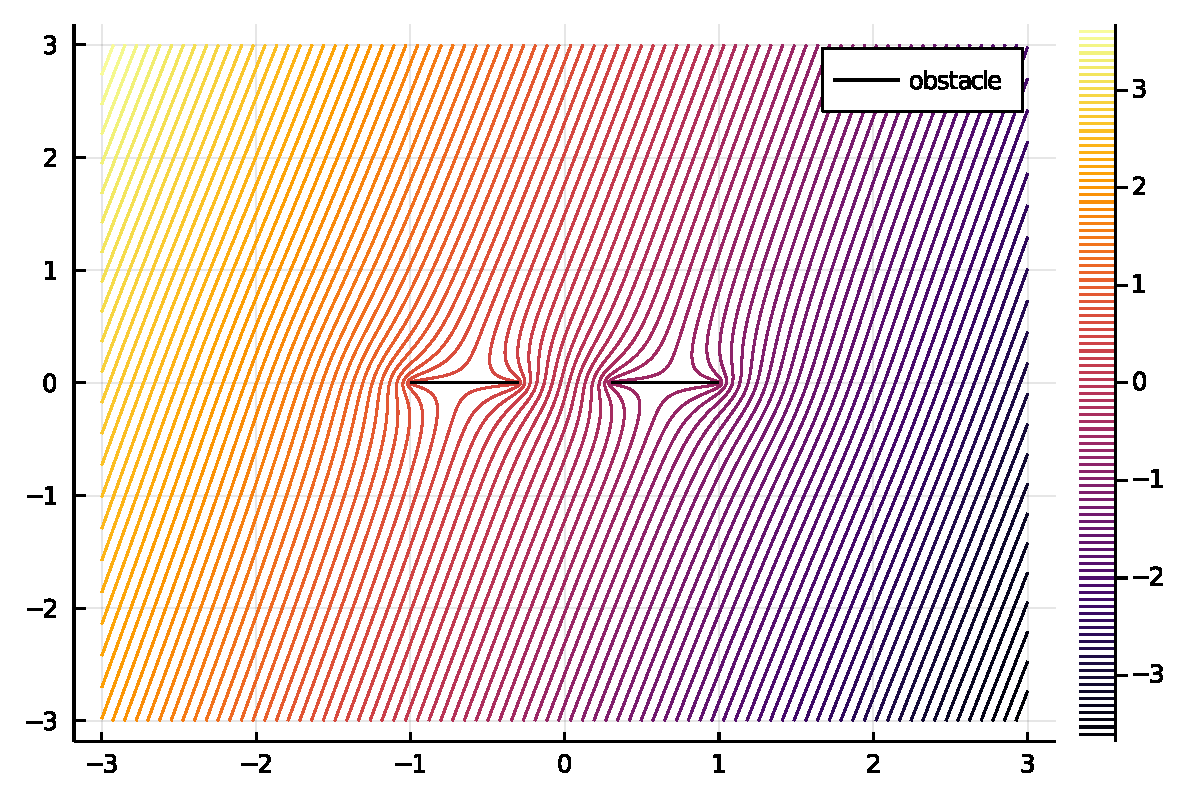
\includegraphics[width=\linewidth]{C:/Users/mfaso/OneDrive/Documents/GitHub/M3M6AppliedComplexAnalysis/output/figures/Lecture14_3_1.pdf}


\end{document}
